%-------------------------------------------------------------------------------
%                            BAB III
%               		METODOLOGI PENELITIAN
%-------------------------------------------------------------------------------

\chapter{METODOLOGI PENELITIAN}

\section{Alat dan Bahan}
	Alat dan bahan yang digunakan pada penelitian ini terbagi atas perangkat keras dan perangkat lunak yang akan dijelaskan seperti berikut.

	\subsection{Perangkat Keras}
		Perangkat keras yang digunakan secara garis besar terdiri atas kit-kit \emph{Wireless Sensor Network} (WSN) dari \emph{vendor} IQRF dan XBee, dan sebuah \emph{Access Point} (AP) TP-LINK MR3020 yang bertindak sebagai \emph{gateway}. Untuk lebih jelasnya dapat dilihat pada daftar berikut.

		\vspace{-0.5cm}

		\begin{enumerate}[a.]
		\begin{singlespace}
		\itemsep0em
			\item Kit pancar-rima IQRF TR-53B (3 unit),
			\item Kit pengunduh program CK-USB-04 (1 unit),
			\item Kit pengembangan DK-EVAL-03 (2 unit),
			\item Kit pengembangan CK-EVAL-04 (1 unit),
			\item \emph{XBee 802.15.4 Radios (Series 1)} (3 unit),
			\item \emph{XBee Explorer USB Board} (1 unit),
			\item \emph{2 channel Relay Shield For Arduino (With XBee/BTBee interface)} (2 unit),
			\item Arduino Uno (2 unit),
			\item TP-LINK MR3020 (1 unit),
			\item Kabel USB ke Serial Prolific (1 unit).
		\end{singlespace}
		\end{enumerate}

	\subsection{Perangkat Lunak}
		Perangkat lunak yang digunakan terdiri atas perangkat lunak yang digunakan untuk mengembangkan aplikasi dan perangkat lunak yang digunakan untuk men-\emph{deploy} aplikasi pada AP. Daftar berikut menjelaskan secara lebih detail tentang aplikasi yang digunakan.

		\vspace{-0.5cm}

		\begin{enumerate}[a.]
		\begin{singlespace}
		\itemsep0em
			\item Arduino for Mac OS X,
			\item CoolTerm,
			\item Driver FTDI for Mac OS X,
			\item PHP, MySQL, dan uHTTPd,
			\item Python dan pustaka PySerial,
			\item IQRF IDE v 2.08 for TR-53B,
			\item SSHFS,
			\item Sublime Text 3.
		\end{singlespace}
		\end{enumerate}

\section{Alur Penelitian}
	\subsection{Pra Penelitian}
		Sebelum penelitian dimulai, dilakukan studi literatur terkait dengan sistem yang akan dibangun. Selain itu, analisis kebutuhan juga dirancang pada tahap ini. Setelah semua selesai, dilajutkan dengan penulisan proposal penelitian.

	\subsection{Pengembangan Aplikasi}
		Ada tiga aplikasi yang akan dibangun, yaitu aplikasi berbasis bahasa C untuk masing-masing sensor IQRF dan Arduino Uno, aplikasi berbasis web yang nantinya akan berinteraksi langsung dengan pengguna, dan aplikasi berbasis bahasa Python untuk mengomunikasikan sensor-sensor dengan aplikasi berbasis web seperti yang diilustrasikan pada Gambar \ref{aplikasi}.

			\begin{figure}[H]
			  \centering
			    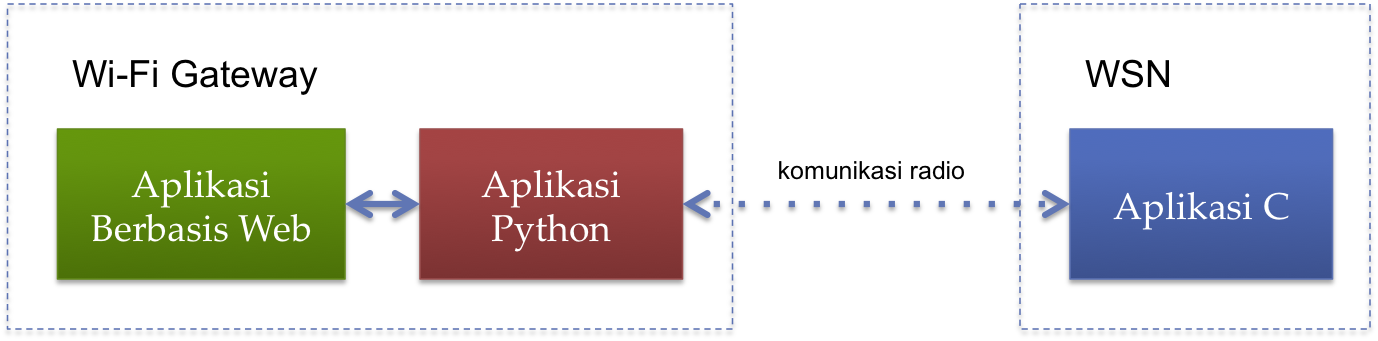
\includegraphics[width=0.9\textwidth]{gambar/aplikasi}
			    \caption{Diagram ilustrasi aplikasi yang dibangun.}
			    \label{aplikasi}
			\end{figure}

		Seperti yang dapat dilihat pada Gambar \ref{aplikasi}, aplikasi berbasis web dan aplikasi Python berjalan pada AP, sedangakan aplikasi C berjalan pada masing-masing sensor IQRF dan XBee (lebih tepatnya Arduino Uno).

		\subsubsection{Pendekatan Interoperabilitas} \
		
		Secara lebih detil, ilustrasi komponen-komponen sistem yang dibangun beserta alur komunikasi dari masing-masing bagian dapat dilihat pada Gambar berikut.

			\begin{figure}[H]
			  \centering
			    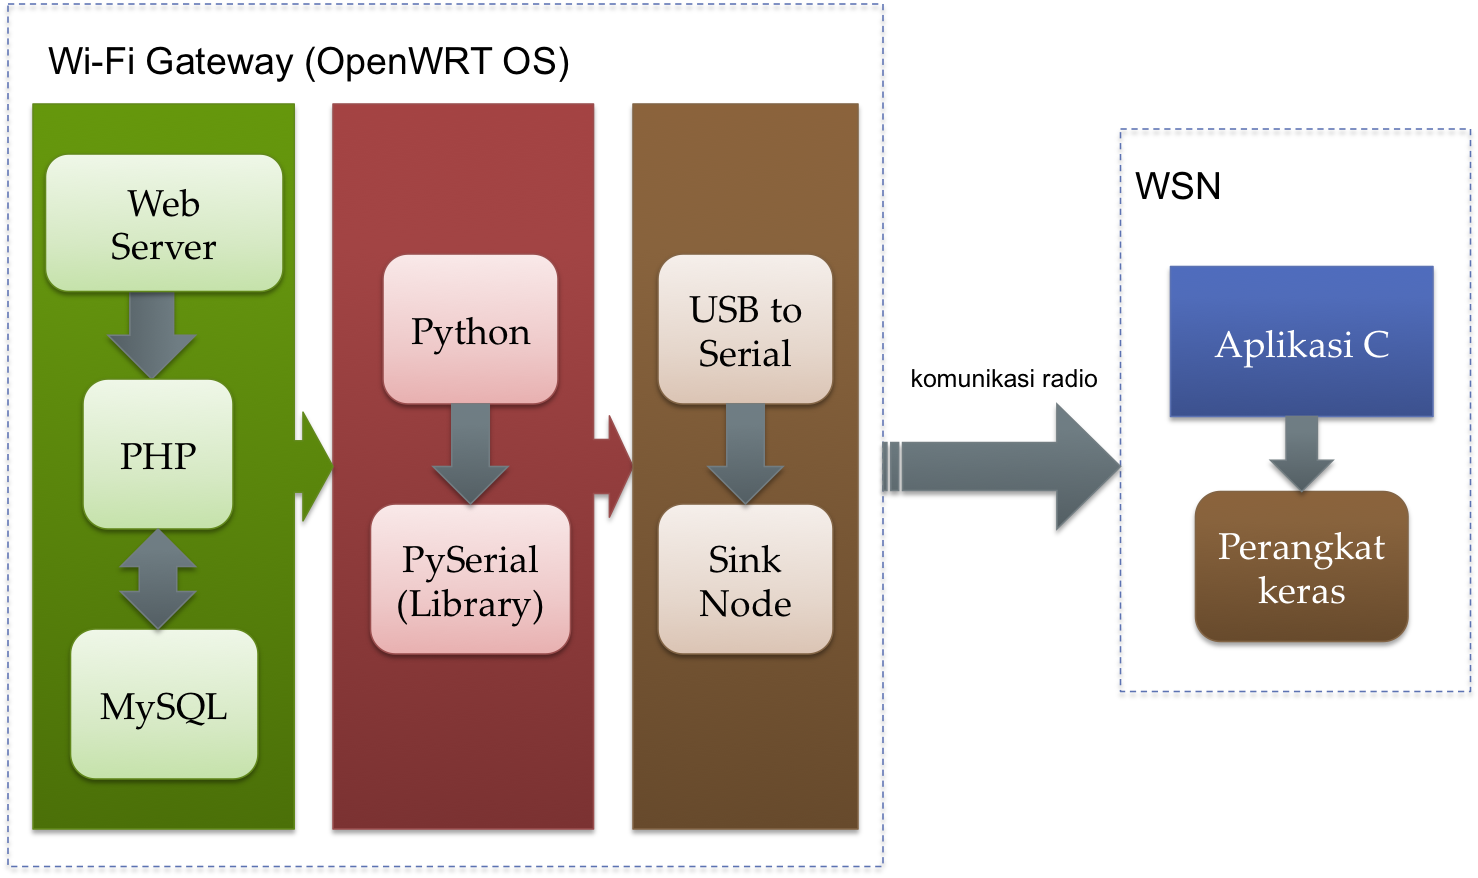
\includegraphics[width=0.9\textwidth]{gambar/communication}
			    \caption{Diagram ilustrasi detil komponen-komponen dari sistem beserta alur komunikasinya.}
			    \label{communication}
			\end{figure}

		Gambar \ref{communication} menggambarkan pendekatan interoperabilitas yang dilakukan pada penelitian ini. Seperti yang dapat dilihat pada Gambar \ref{communication}, komunikasi antara \emph{sink-node} dan aplikasi web (warna hijau) dijembatani oleh USB \emph{to serial} dan aplikasi Python. Hal ini dimungkinkan karena masing-masing \emph{sink-node} dari WSN sama-sama menggunakan komunikasi data serial untuk bertukar informasi dengan \emph{gateway}. Pada pendekatan ini, seluruh aplikasi yang dirancang berjalan di atas sistem operasi OpenWrt. Pendekatan ini dapat menginteroperabilitaskan beberapa WSN dengan hanya satu buah \emph{gateway}.

		Pendekatan interoperabilitas WSN yang lain dapat dilakukan dengan menggunakan \emph{gateway} internet dari masing-masing vendor. Pendekatan ini akan akan memanfaatkan \emph{web-service} yang tersedia di masing-masing vendor untuk diinteroperabilitaskan. Namun demikian, untuk menempuh pendekatan ini, diperlukan biaya yang tinggi karena harga dari masing-masing \emph{gateway} internet WSN berkisar di angka ratusan Dolar Amerika Serikat atau jutaan Rupiah. Oleh karena itu, pendekatan ini sangat bertolak belakang dengan tujuan penelitian ini yang mengedepankan sisi rendah biaya (\emph{low-cost}) sehingga pendekatan ini tidak dilakukan. Selain itu, faktor ketertutupan dari \emph{gateway} internet WSN juga menjadi kelemahan dari pilihan ini karena hal ini akan menyulitkan jika \emph{web-service} yang telah tersedia kurang memenuhi kebutuhan dan diinginkan modifikasi \emph{gateway}. \\ \\

		\subsubsection{Teknis Pengembangan} \

		Aplikasi untuk sensor-sensor IQRF terdiri dari dua bagian, yaitu aplikasi untuk sensor koordinator dan sensor simpul. Namun demikian, aplikasi sama-sama ditulis dan kembangkan menggunakan Sublime Text 3. Setelah kode sumber untuk aplikasi selesai dibuat, kode sumber dikompiliasi menggunakan IDE IQRF untuk kemudian diunggah ke sensor menggunakan bantuan aplikasi yang sama. Aplikasi yang dikembangkan adalah hasil fork dari iHome, aplikasi rumah hijau yang dikembangkan oleh \cite{widyawan2012ihome}.

		Sedangkan aplikasi untuk Arduino Uno, yang bertugas menyala-matikan relay dengan komunikasi berbasis ZigBee, dikembangkan dengan aplikasi Arduino for Mac OS X dengan bahasa pemrograman C. Proses kompilasi dan pengunggahan dilakukan dengan bantuan aplikasi yang sama.

		Aplikasi web dikembangkan dengan bahasa PHP pada server (terletak pada AP) dan JavaScript pada klien. Halaman yang tertampil pada web browser disusun menggunakan HTML5 dan CSS3 dengan bantuan pustaka Bootstrap agar halaman dapat bersifat responsif, yaitu dapat menyesuaikan tampilan sesuai ukuran layar web browser. AJAX diterapkan dalam pengembangan agar halaman web yang ditampilkan bersifat dinamis.

		Aplikasi berbasis bahasa Python dikembangkan dengan bantuan pustaka (\emph{library}) PySerial. Pustaka ini diperlukan agar Python dapat berkomunikasi dengan \emph{port} serial, yaitu antar muka untuk berkomunikasi dengan sensor. Kode sumber ditulis menggunakan Sublime Text 3.

	\subsection{Evaluasi dan Perbaikan}
		Evaluasi dilakukan dengan melakukan simulasi dalam skala laboratorium. Simulasi yang diujikan mencakup semua fitur yang dimiliki oleh aplikasi untuk memastikan bahwa aplikasi dapat berjalan dengan semestinya. Kemudian Perbaikan dilakukan dengan bantuan SSHFS agar AP dapat mengakses direktori yang tersimpan pada komputer karena \emph{coding} tidak dilakukan pada AP itu sendiri, melainkan komputer. Perbaikan dilakukan pada komputer karena OpenWRT tidak memiliki antar muka berbasis grafis \emph{Graphical User Interface}.

	\subsection{Pasca Penelitian}
		Setelah penelitian selesai dilakukan dan aplikasi siap untuk diimplementasikan, naskah skripsi dan makalah skripsi ditulis sebagai manifesto penelitian.

	\subsection{Diagram Alir Penelitian}
		Diagram alir penelitian yang menjelaskan tentang alur pekerjaan penelitian dapat dilihat pada Gambar \ref{flowchart-penelitian}.

		\begin{figure}[H]
		  \centering
		    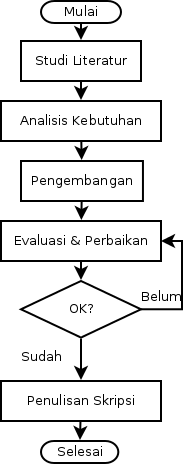
\includegraphics[width=0.3\textwidth]{gambar/flowchart}
		    \caption{Diagram alir penelitian.}
		    \label{flowchart-penelitian}
		\end{figure}

		Pada Gambar \ref{flowchart-penelitian}, dapat dilihat bahwa penelitian dilakukan dengan urutan studi literatur, analisis kebutuhan, pengembangan, iterasi perbaikan dan evaluasi, dan diakhiri dengan penulisan skripsi.


\section{Tahapan Pelaksanaan}
	Rancangan arsitektur yang akan digunakan pada penelitian ini diilustrasikan seperti pada Gambar \ref{wifi}. Pada gambar tersebut diilustrasikan sebuah sistem yang terdiri atas dua buah WSN dengan protokol yang berbeda dan satu buah jaringan nirkabel lokal (WiFi). Protokol WSN yang akan digunakan dalam penelitian ini adalah dari IQRF dan ZigBee. Pelaksanaan penelitian ini akan dibagi menjadi tiga paket pekerjaan atau \emph{Work Package} (WP).

	\noindent\textbf{WP 1: Perancangan Perangkat Lunak}

	Pada tahap ini akan dilakukan studi literatur yang dititikberatkan pada sistem operasi untuk piranti tertanam (\emph{embedded device}). Langkah selanjutnya adalah rerancangan perangkat lunak yang akan ditanamkan pada \emph{Access Point} (AP). Perangkat lunak yang akan ditanamkan harus bekerja secara efisien karena kemampuan komputasi yang terbatas pada AP.

		\begin{figure}[ht!]
		  \centering
		    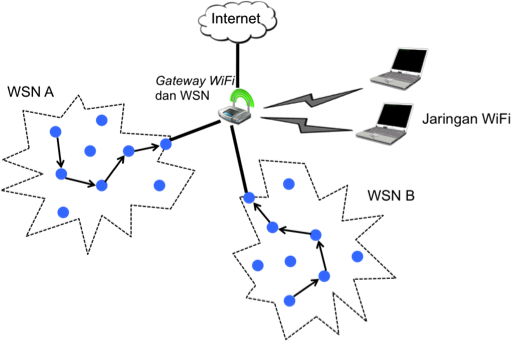
\includegraphics[width=0.9\textwidth]{gambar/wifi}
		    \caption{Arsitektur WSN dan WiFi dengan sebuah AP.}
		    \label{wifi}
		\end{figure}

	\noindent\textbf{WP 2: Implementasi Perangkat Lunak}

	Implementasi perangkat lunak dilakukan pada tahap ini. Langkah pertama yang dilakukan adalah memastikan bahwa WSN dapat terhubungan dengan internet sesuai dengan yang direncanakan. Langkah selanjutnya adalah memastikan bahwa jaringan WiFi tidak mengalami gangguan setelah perangkat lunak yang baru tertanam pada AP. Penambahan layanan-layanan yang diperlukan dapat pula dilakukan pada tahap ini.

	\noindent\textbf{WP 3: Integrasi dan Pengujian Seluruh Sistem}

	Jika jaringan WiFi dan dua protokol WSN masing-masing dapat berhubungan dengan internet, maka pada tahap ini akan dilakukan pengujian sistem secara keseluruhan. Pengujian dinaikkan dari skala lab menjadi skala \emph{test-bed}. Pengujian dalam \emph{test-bed} dilakukan untuk menjamin bahwa sistem yang dikembangkan bekerja sesuai dengan yang direncanakan.


\section{Jadwal Kegiatan}
	Penelitian direncanakan akan dilaksanakan selama enam bulan. Rincian rencana jadwal penelitian dicantumkan dalam Tabel \ref{jadwal}.

	% Please remember to add \use{multirow} to your document preamble in order to suppor multirow cells
		\begin{table}[H]
		\centering
		\caption{Jadwal Penelitian.}
		\label{jadwal}
		\begin{tabular}{|c|l|l|l|l|l|l|l|}
		\hline
		\multirow{2}{*}{No} & \multirow{2}{*}{Keterangan} & \multicolumn{6}{c|}{Bulan}                                                                                                                          \\ \cline{3-8} 
		                    &                             & 1 & 2 & 3 & 4 & 5 & 6 \\ \hline
		1                   & Studi literatur                                  &\cellcolor{gray} &\cellcolor{gray}&                        &                        &                        &                         \\ \hline
		2                   & Desain                                           &                        &\cellcolor{gray}&\cellcolor{gray}&                        &                        &                         \\ \hline
		3                   & Pembelian bahan                                  &                        &                        &\cellcolor{gray}&                        &                        &                         \\ \hline
		4                   & Pembuatan prototipe                              &                        &                        &\cellcolor{gray}&\cellcolor{gray}&\cellcolor{gray}&                         \\ \hline
		5                   & Uji coba dan perbaikan                           &                        &                        &                        &\cellcolor{gray}&\cellcolor{gray}&                         \\ \hline
		6                   & Penulisan skripsi                                &                        &                        &                        &                        &                        &\cellcolor{gray}\\ \hline
		\end{tabular}
		\end{table}
	
% Baris ini digunakan untuk membantu dalam melakukan sitasi
% Karena diapit dengan comment, maka baris ini akan diabaikan
% oleh compiler LaTeX.
\begin{comment}
\bibliography{daftar-pustaka}
\end{comment}
